\chapter{Arhitektura i dizajn sustava}

		Arhitektura je podijeljena na tri podsustava:
    \begin{packed_item}
        \item Mobilna aplikacija
        \item Poslužitelj
        \item Poslužitelj baze podataka
    \end{packed_item}
    
    Okviri i jezici koristimo izabrani su imajući na umu, između ostaloga, njihovu relativno dugotrajnu popularnost, što znači da osim male vjerojatnosti skore zastare postoji i veliki skup korisnika koji pružaju podršku, kao i problema koje su ti korisnici već riješili, a dostupni su na stranicama poput \url{stackoverflow.com}. Također su izvrsno dokumentirani. \\
    
	    \begin{figure}[H]
	        \begin{center}
            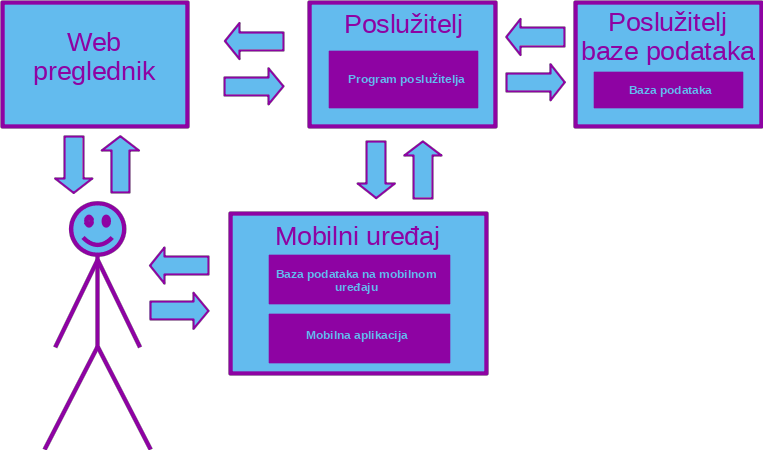
\includegraphics[width=1.0\linewidth]{slike/arh_skica.png}
            \caption{Skica arhitekture sustava}
            \label{fig:arh_skica}
            \end{center}
        \end{figure}
        
    \underbar{Aplikacija na mobilnom uređaju} napravljena je za sustav Android. Dio je frontend sloja, ali i u sklopu operativnog sustava komunicira s ugrađenom lokalnom bazom podataka (dakle nema zasebni poslužitelj). Preko protokola HTTP komunicira s poslužiteljem. Mobilna aplikacija napisana je u strojno podržanom (native) jeziku Androida - Java - koji je objektno orijentirani jezik što nam omogućuje podjelu u razrede koji su u paketima grupirani u međusobno povezane elemente, a pritom nam omogućuje i zadržavanje apstrakcije. Omogućuje nam i ponovnu iskoristivost jer bilo koji uređaj koji ima Java virtualni stroj može pokrenuti isti kôd. Android kao programski okvir omogućava veliku fleksibilnost (kroz razmještanje i imenovanje resursa prema dogovoru), poput automatske promjene jezika ovisno o korisničkim postavkama ili rezolucije slika ovisno o rezoluciji ekrana. \\
    \underbar{Kôd na poslužitelju} dio je backend sloja i napisan je u Pythonu 3 koji se, osim spomenutim prednostima objektno orijentirane paradigme, odlikuje i jednostavnošću kodiranja što značajno smanjuje vrijeme razvoja. Pogotovo uz backend okvir \textit{django} koji omogućava fleksibilnost ne koristeći "Convention over configuration" paradigmu, ali je i dalje jednostavan jer je pisan u Pythonu. Njegovo svojstvo "batteries included" smanjuje količinu posla razvojnom timu akcijama poput automatskog stvaranja sučelja za administratora kojemu se može pristupiti iz \underbar{web preglenika} korištenjem HTTP protokola te jednostavnog povezivanja s email poslužiteljem pomoću SMTP protokola. \\
    Koristimo stilističku varijaciju arhitekture zasnovane na događajima: MVC (\textit{Model, View, Controller}) obrazac. Kako mu i ime kaže, dijeli aplikaciju na model, pogled (View) i nadglednik (Controller). Time se omogućava odvajanje korisničkog sučelja (kroz pogled) od ostatka sustava. Za upravljanje zahtjevima korisnika služi nadglednik, a model opisuje strukturu i pravila vezane uz podatke. Podržava ga django. \\
  
	
		

		

				
		\section{Baze podataka}
		
		Za spremanje podataka koristimo, zbog njihove uvriježenosti i uglavnom velike sličnosti s našim poimanjem onoga što predstavljaju, relacijske baze podataka. One dijele informacije o objektima u atribute, a vrste objekata u tablice, tj. relacije. Takve baze podataka upravo postoje i optimirane su za učinkovito spremanje čitanje i izmjenu podatka, pa ih zato za to i koristimo. Konkretno, na poslužitelju smo se odlučili za PostgreSQL, a na Android uređaju imamo SQLite3. \\
		
		Slijede opisi tablica i njihovih veza. Imena atributa primarnog ključa deblje su otisnuta, a pozadinska boja ćelije u kojoj je ime stranog ključa promijenjena je u plavu.
			
			
		%--------------------------------------------------------------------------------
		

            \subsection{Opis tablica na uređaju}

                Tablica \underbar{omiljeni} sadrži šifre stavaka koje su označene kao omiljene. Tablica omiljeni je u \textit{Many-to-one} vezi s tablicom stavka (preko atributa sifStavka).
                \begin{longtabu} to \textwidth {|X[6, l]|X[6, l]|X[20, l]|}
                    
                    \hline \multicolumn{3}{|c|}{\textbf{omiljeni}}     \\[3pt] \hline
                    \endfirsthead
                    
                    \hline \multicolumn{3}{|c|}{\textbf{omiljeni}}     \\[3pt] \hline
                    \endhead
                    
                    \hline 
                    \endlastfoot

                    \cellcolor{LightBlue} \textbf{sifStavka} & INT & šifra stavke koja je označena kao omiljena \\ \hline
                    
                    
                    
                \end{longtabu}

                Tablica \underbar{popis} sadrži nazive popisa i njihove načine izračuna cijene. Tablica popis je u \textit{One-to-many} vezi s tablicom stavka (preko atributa sifPopis).
                \begin{longtabu} to \textwidth {|X[6, l]|X[6, l]|X[20, l]|}
                    
                    \hline \multicolumn{3}{|c|}{\textbf{popis}}     \\[3pt] \hline
                    \endfirsthead
                    
                    \hline \multicolumn{3}{|c|}{\textbf{popis}}     \\[3pt] \hline
                    \endhead
                    
                    \hline 
                    \endlastfoot

                    \textbf{sifPopis} & INT & šifra popisa \\ \hline
                    nazivPopis & NCHAR VARYING & naziv popisa \\ \hline
                    izrCijene & BIT & način izračuna cijene \\ \hline
                    sifTrgovina & INT & šifra trgovine vezane uz popis (ako je primjenjivo) \\ \hline
                    
                    
                    
                \end{longtabu}

                Tablica \underbar{stavka} sadrži stavke na popisu. Tablica stavka je u \textit{One-to-many} vezi s tablicom omiljeni (preko atributa sifStavka). Tablica stavka je u \textit{Many-to-one} vezi s tablicom popis (preko atributa sifPopis).
                \begin{longtabu} to \textwidth {|X[6, l]|X[6, l]|X[20, l]|}
                    
                    \hline \multicolumn{3}{|c|}{\textbf{stavka}}     \\[3pt] \hline
                    \endfirsthead
                    
                    \hline \multicolumn{3}{|c|}{\textbf{stavka}}     \\[3pt] \hline
                    \endhead
                    
                    \hline 
                    \endlastfoot

                    \textbf{sifStavka} & INT & šifra stavke \\ \hline
                    \cellcolor{LightBlue} sifPopis & INT & šifra popisa na kojem je stavka \\ \hline
                    barkod & DECIMAL & barkod artikla \\ \hline
                    cijena & DECIMAL & cijena artikla \\ \hline
                    filtarFunkcija & VARCHAR & sadrži sažeto napisane filtar funkcije koje se primjenjuju \\ \hline
                    uKosarici & BIT & oznaka je li stavka dodana u košaricu \\ \hline
                    kolicina & DECIMAL & količina artikla u intervalu [0,000 - 999,999] \\ \hline
                    naziv & NCHAR VARYING & naziv artikla \\ \hline
                    sifTrgovina & INT & šifra trgovine vezane uz cijenu \\ \hline
                    
                    
                    
                \end{longtabu}



            \subsection{Opis tablica na posluzitelju}

                Tablica \underbar{artikl} sadrži popis svih barkodova artikala. Tablica artikl je u \textit{One-to-many} vezi s tablicom opisArtikla (preko atributa barkod) i tablicom artiklUTrgovini (preko atributa barkod).
                \begin{longtabu} to \textwidth {|X[6, l]|X[6, l]|X[20, l]|}
                    
                    \hline \multicolumn{3}{|c|}{\textbf{artikl}}     \\[3pt] \hline
                    \endfirsthead
                    
                    \hline \multicolumn{3}{|c|}{\textbf{artikl}}     \\[3pt] \hline
                    \endhead
                    
                    \hline 
                    \endlastfoot

                    \textbf{barkod} & DECIMAL & barkod artikla \\ \hline
                    
                    
                    
                \end{longtabu}

                Tablica \underbar{artiklUTrgovini} sadrži popis artikala u trgovini. Tablica artiklUTrgovini je u \textit{Many-to-one} vezi s tablicom artikl (preko atributa barkod), tablicom trgovina (preko atributa sifTrgovina) i tablicom opisArtikla (preko atributa barkod i email).
                \begin{longtabu} to \textwidth {|X[6, l]|X[6, l]|X[20, l]|}
                    
                    \hline \multicolumn{3}{|c|}{\textbf{artiklUTrgovini}}     \\[3pt] \hline
                    \endfirsthead
                    
                    \hline \multicolumn{3}{|c|}{\textbf{artiklUTrgovini}}     \\[3pt] \hline
                    \endhead
                    
                    \hline 
                    \endlastfoot

                    \cellcolor{LightBlue} \textbf{barkod} & DECIMAL & barkod artikla \\ \hline
                    \cellcolor{LightBlue} \textbf{sifTrgovina} & CHAR & šifra trgovine \\ \hline
                    \cellcolor{LightBlue} email & VARCHAR & email vezan uz željeni opis \\ \hline
                    cijena & DECIMAL & cijena artikla u trgovini \\ \hline
                    popust & FLOAT & popust na cijenu artikla u trgovini \\ \hline
                    dostupnost & BIT & ima li artikla u trgovini \\ \hline
                    
                    
                    
                \end{longtabu}

                Tablica \underbar{kategorija} sadrži popis kategorija artikala. Tablica kategorija je u \textit{One-to-many} vezi s tablicom potkategorija (preko atributa sifKategorija).
                \begin{longtabu} to \textwidth {|X[6, l]|X[6, l]|X[20, l]|}
                    
                    \hline \multicolumn{3}{|c|}{\textbf{kategorija}}     \\[3pt] \hline
                    \endfirsthead
                    
                    \hline \multicolumn{3}{|c|}{\textbf{kategorija}}     \\[3pt] \hline
                    \endhead
                    
                    \hline 
                    \endlastfoot

                    \textbf{sifKategorija} & INT & šifra kategorije artikla \\ \hline
                    nazivKategorija & NCHAR VARYING & naziv kategorije artikla \\ \hline
                    
                    
                    
                \end{longtabu}

                Tablica \underbar{korisnik} sadrži informacije o prijavljenim korisnicima aplikacije. Tablica korisnik je u \textit{One-to-many} vezi s tablicom onemoguceniRacun (preko atributa email), tablicom opisArtikla (preko atributa email), tablicom privremenaLozinka (preko atributa email) i tablicom trgovina (preko atributa email). Tablica korisnik je u \textit{Many-to-one} vezi s tablicom uloga (preko atributa sifUloga).
                \begin{longtabu} to \textwidth {|X[6, l]|X[6, l]|X[20, l]|}
                    
                    \hline \multicolumn{3}{|c|}{\textbf{korisnik}}     \\[3pt] \hline
                    \endfirsthead
                    
                    \hline \multicolumn{3}{|c|}{\textbf{korisnik}}     \\[3pt] \hline
                    \endhead
                    
                    \hline 
                    \endlastfoot

                    \textbf{email} & VARCHAR & email korisnika \\ \hline
                    \cellcolor{LightBlue} sifUloga & INT & šifra uloge korisnika \\ \hline
                    lozinka & VARCHAR & hash lozinke korisnika (SHA 256) \\ \hline
                    token & CHAR & token sjednice korisnika \\ \hline
                    
                    
                    
                \end{longtabu}

                Tablica \underbar{onemoguceniRacun} sadrži popis onemogućenih računa. Tablica onemoguceniRacun je u \textit{Many-to-one} vezi s tablicom korisnik (preko atributa adminEmail).
                \begin{longtabu} to \textwidth {|X[6, l]|X[6, l]|X[20, l]|}
                    
                    \hline \multicolumn{3}{|c|}{\textbf{onemoguceniRacun}}     \\[3pt] \hline
                    \endfirsthead
                    
                    \hline \multicolumn{3}{|c|}{\textbf{onemoguceniRacun}}     \\[3pt] \hline
                    \endhead
                    
                    \hline 
                    \endlastfoot

                    \cellcolor{LightBlue} \textbf{onemoguceni} & VARCHAR & email osobe kojoj je onemogućen pristup \\ \hline
                    \cellcolor{LightBlue} \textbf{adminEmail} & VARCHAR & email admina koji je onemogućio osobi pristup \\ \hline
                    datum & DATE & datum onemogućenja \\ \hline
                    
                    
                    
                \end{longtabu}

                Tablica \underbar{opisArtikla} sadrži opis i informacije vezane uz artikl zadan barkodom koje je napisao neki prijavljeni korisnik. Tablica opisArtikla je u \textit{One-to-many} vezi s tablicom artiklUTrgovini (preko atributa barkod i email). Tablica opisArtikla je u \textit{Many-to-one} vezi s tablicom artikl (preko atributa barkod), tablicom korisnik (preko atributa email), tablicom vrsta (preko atributa sifKategorija, sifPotkategorija i sifVrsta) i tablicom zemlja (preko atributa sifZemlja).
                \begin{longtabu} to \textwidth {|X[6, l]|X[6, l]|X[20, l]|}
                    
                    \hline \multicolumn{3}{|c|}{\textbf{opisArtikla}}     \\[3pt] \hline
                    \endfirsthead
                    
                    \hline \multicolumn{3}{|c|}{\textbf{opisArtikla}}     \\[3pt] \hline
                    \endhead
                    
                    \hline 
                    \endlastfoot

                    \cellcolor{LightBlue} \textbf{barkod} & DECIMAL & barkod artikla \\ \hline
                    \cellcolor{LightBlue} \textbf{email} & VARCHAR & email osobe koja je napisala opis \\ \hline
                    \cellcolor{LightBlue} sifKategorija & INT & šifra kategorije artikla \\ \hline
                    \cellcolor{LightBlue} sifPotkategorija & INT & šifra potkategorije artikla \\ \hline
                    \cellcolor{LightBlue} sifVrsta & INT & šifra vrste artikla \\ \hline
                    \cellcolor{LightBlue} sifZemlja & CHAR & šifra zemlje podrijetla \\ \hline
                    kratkiOpis & NCHAR VARYING & kratki opis artikla (do 255 znakova) \\ \hline
                    nazivArtikla & NCHAR VARYING & naziv artikla (do 32 znaka) \\ \hline
                    brojGlasova & INT & broj glasova o opisu artikla (goreglasovi - doljeglasovi) \\ \hline
                    masa & INT & masa artikla \\ \hline
                    
                    
                    
                \end{longtabu}

                Tablica \underbar{potkategorija} sadrži popis potkategorija artikala. Tablica potkategorija je u \textit{One-to-many} vezi s tablicom vrsta (preko atributa sifKategorija i sifPotkategorija). Tablica potkategorija je u \textit{Many-to-one} vezi s tablicom kategorija (preko atributa sifKategorija).
                \begin{longtabu} to \textwidth {|X[6, l]|X[6, l]|X[20, l]|}
                    
                    \hline \multicolumn{3}{|c|}{\textbf{potkategorija}}     \\[3pt] \hline
                    \endfirsthead
                    
                    \hline \multicolumn{3}{|c|}{\textbf{potkategorija}}     \\[3pt] \hline
                    \endhead
                    
                    \hline 
                    \endlastfoot

                    \cellcolor{LightBlue} \textbf{sifKategorija} & INT & šifra kategorije kojoj potkategorija artikla pripada \\ \hline
                    \textbf{sifPotkategorija} & INT & šifra podkategorije artikla \\ \hline
                    nazivPotkategorija & NCHAR VARYING & naziv potkategorije artikla \\ \hline
                    
                    
                    
                \end{longtabu}

                Tablica \underbar{privremenaLozinka} sadrži privremene lozinke poslane na email korisnika. Tablica privremenaLozinka je u \textit{Many-to-one} vezi s tablicom korisnik (preko atributa email).
                \begin{longtabu} to \textwidth {|X[6, l]|X[6, l]|X[20, l]|}
                    
                    \hline \multicolumn{3}{|c|}{\textbf{privremenaLozinka}}     \\[3pt] \hline
                    \endfirsthead
                    
                    \hline \multicolumn{3}{|c|}{\textbf{privremenaLozinka}}     \\[3pt] \hline
                    \endhead
                    
                    \hline 
                    \endlastfoot

                    \cellcolor{LightBlue} \textbf{email} & VARCHAR & email korisnika koji je zatrazio promjenu \\ \hline
                    lozinka & CHAR & hash privremene lozinke \\ \hline
                    istice & DATE & datum isteka lozinke \\ \hline
                    
                    
                    
                \end{longtabu}

                Tablica \underbar{tajniBroj} sadrži popis tajnih brojeva za registraciju. Tablica tajniBroj je u \textit{Many-to-one} vezi s tablicom uloga (preko atributa sifUloga).
                \begin{longtabu} to \textwidth {|X[6, l]|X[6, l]|X[20, l]|}
                    
                    \hline \multicolumn{3}{|c|}{\textbf{tajniBroj}}     \\[3pt] \hline
                    \endfirsthead
                    
                    \hline \multicolumn{3}{|c|}{\textbf{tajniBroj}}     \\[3pt] \hline
                    \endhead
                    
                    \hline 
                    \endlastfoot

                    \textbf{broj} & INT & tajni broj \\ \hline
                    \cellcolor{LightBlue} sifUloga & INT & šifra uloge koju će korisnik poprimiti \\ \hline
                    idKorisnika & INT & neki identifikator osobe koja će iskoristiti tajni broj \\ \hline
                    
                    
                    
                \end{longtabu}

                Tablica \underbar{trgovina} sadrži informacije o trgovinama. Tablica trgovina je u \textit{One-to-many} vezi s tablicom artiklUTrgovini (preko atributa sifTrgovina). Tablica trgovina je u \textit{Many-to-one} vezi s tablicom korisnik (preko atributa email).
                \begin{longtabu} to \textwidth {|X[6, l]|X[6, l]|X[20, l]|}
                    
                    \hline \multicolumn{3}{|c|}{\textbf{trgovina}}     \\[3pt] \hline
                    \endfirsthead
                    
                    \hline \multicolumn{3}{|c|}{\textbf{trgovina}}     \\[3pt] \hline
                    \endhead
                    
                    \hline 
                    \endlastfoot

                    \textbf{sifTrgovina} & CHAR & šiftra trgovine \\ \hline
                    \cellcolor{LightBlue} email & VARCHAR & email vlasnika trgovine \\ \hline
                    lat & DECIMAL & geografska širina trgovine \\ \hline
                    lon & DECIMAL & geografska dužina trgovine \\ \hline
                    nazivTrgovina & NCHAR & naziv trgovine \\ \hline
                    adresa & VARCHAR & adresa trgovine \\ \hline
                    radnoVrijemePoc & TIME & početak radnog vremena trgovine \\ \hline
                    radnoVrijemeKraj & TIME & kraj radnog vremena \\ \hline
                    
                    
                    
                \end{longtabu}

                Tablica \underbar{uloga} sadrži popis uloga koje prijavljeni korisnik može poprimiti (administrator, trgovac ili kupac). Tablica uloga je u \textit{One-to-many} vezi s tablicom korisnik (preko atributa sifUloga) i tablicom tajniBroj (preko atributa sifUloga).
                \begin{longtabu} to \textwidth {|X[6, l]|X[6, l]|X[20, l]|}
                    
                    \hline \multicolumn{3}{|c|}{\textbf{uloga}}     \\[3pt] \hline
                    \endfirsthead
                    
                    \hline \multicolumn{3}{|c|}{\textbf{uloga}}     \\[3pt] \hline
                    \endhead
                    
                    \hline 
                    \endlastfoot

                    \textbf{sifUloga} & INT & šifra uloge korisnika \\ \hline
                    nazUloga & VARCHAR & naziv uloge prijavljenog korisnika \\ \hline
                    
                    
                    
                \end{longtabu}

                Tablica \underbar{vrsta} sadrži popis vrsta artikala. Tablica vrsta je u \textit{One-to-many} vezi s tablicom opisArtikla (preko atributa sifKategorija, sifPotkategorija i sifVrsta). Tablica vrsta je u \textit{Many-to-one} vezi s tablicom potkategorija (preko atributa sifKategorija i sifPotkategorija).
                \begin{longtabu} to \textwidth {|X[6, l]|X[6, l]|X[20, l]|}
                    
                    \hline \multicolumn{3}{|c|}{\textbf{vrsta}}     \\[3pt] \hline
                    \endfirsthead
                    
                    \hline \multicolumn{3}{|c|}{\textbf{vrsta}}     \\[3pt] \hline
                    \endhead
                    
                    \hline 
                    \endlastfoot

                    \cellcolor{LightBlue} \textbf{sifKategorija} & INT & šifra kategorije kojoj vrsta artikla pripada \\ \hline
                    \cellcolor{LightBlue} \textbf{sifPotkategorija} & INT & šifra potkategorije kojoj vrsta artikla pripada \\ \hline
                    \textbf{sifVrsta} & INT & šifra vrste \\ \hline
                    nazivVrsta & NCHAR VARYING & naziv vrste artikla \\ \hline
                    
                    
                    
                \end{longtabu}

                Tablica \underbar{zemlja} sadrži popis zemalja koje korisnik može odabrati kao zemlju podrijetla. Tablica zemlja je u \textit{One-to-many} vezi s tablicom opisArtikla (preko atributa sifZemlja).
                \begin{longtabu} to \textwidth {|X[6, l]|X[6, l]|X[20, l]|}
                    
                    \hline \multicolumn{3}{|c|}{\textbf{zemlja}}     \\[3pt] \hline
                    \endfirsthead
                    
                    \hline \multicolumn{3}{|c|}{\textbf{zemlja}}     \\[3pt] \hline
                    \endhead
                    
                    \hline 
                    \endlastfoot

                    \textbf{sifZemlja} & CHAR & šifra zemlje podrijetla \\ \hline
                    nazivZemlja & NCHAR VARYING & naziv zemlje podrijetla \\ \hline
                    
                    
                    
                \end{longtabu}

		%------------------------------------------------------------------------------
			\subsection{Dijagrami baze podataka}
		\begin{figure}[H]
		    \centering
			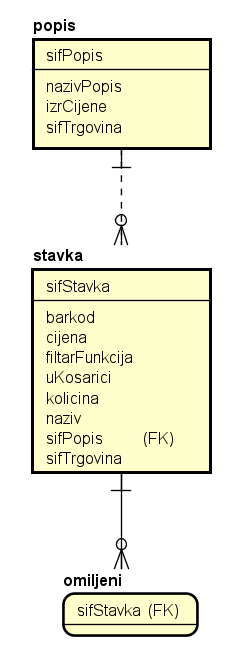
\includegraphics[scale=0.4]{dijagrami/db_uredaj.png}
			\caption{Baza podataka na uređaju}
			\label{fig:db_uredaj}
		\end{figure}
		
		\begin{figure}[H]
		    \centering
			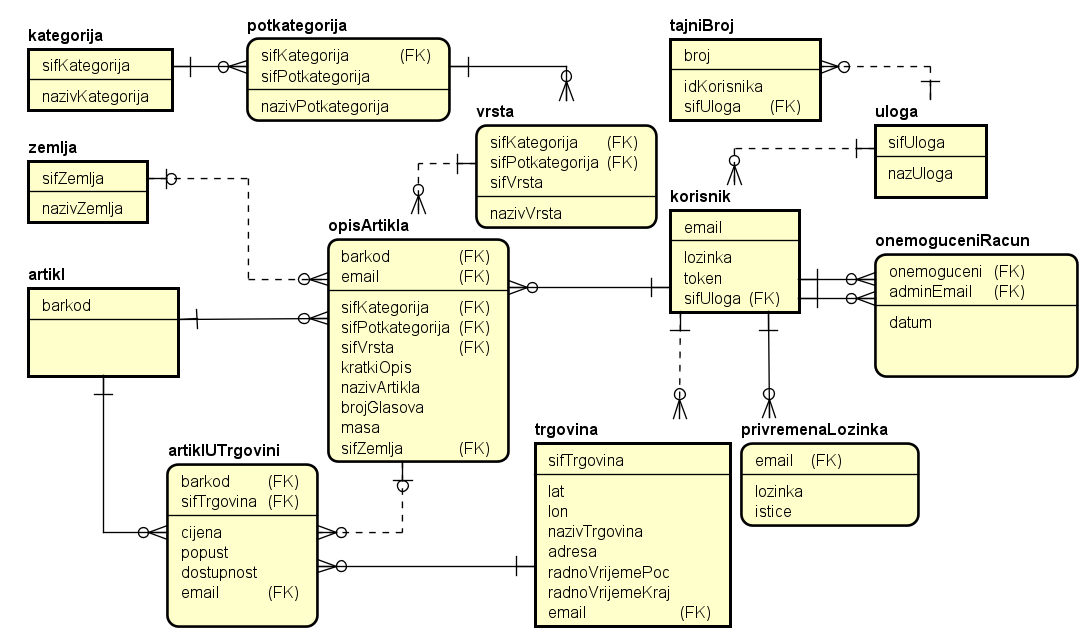
\includegraphics[width=.9\linewidth]{dijagrami/db_posluzitelj.png}
			\caption{Baza podataka na poslužitelju}
			\label{fig:db_posluzitelj}
		\end{figure}
			
			\eject
			
			
		\section{Dijagrami razreda}
		
		Dijagram razreda na uređaju sadrži klase koje nisu dio generične funkcionalnosti, ali su ubačene radi preglednosti. To su List, Listitem, RoomDB, Favourites i About
		
		\begin{figure}[H]
		    \centering
			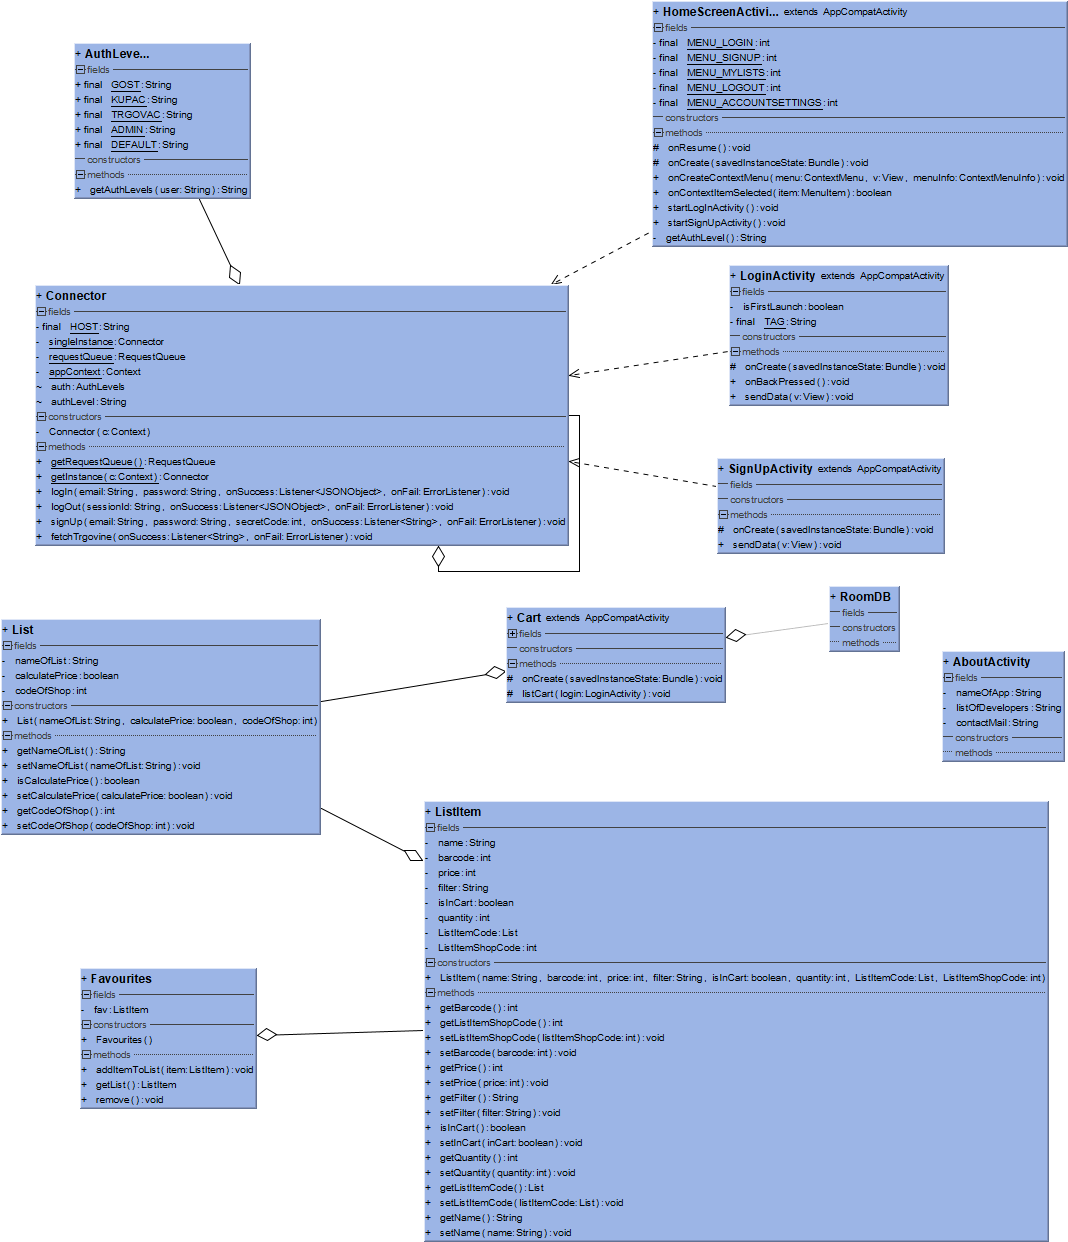
\includegraphics[scale=0.4]{dijagrami/class_uredaj.png}
			\caption{Dijagram razreda na uređaju}
			\label{fig:class_uredaj}
		\end{figure}
		
		
		
		\begin{figure}[H]
		    \centering
			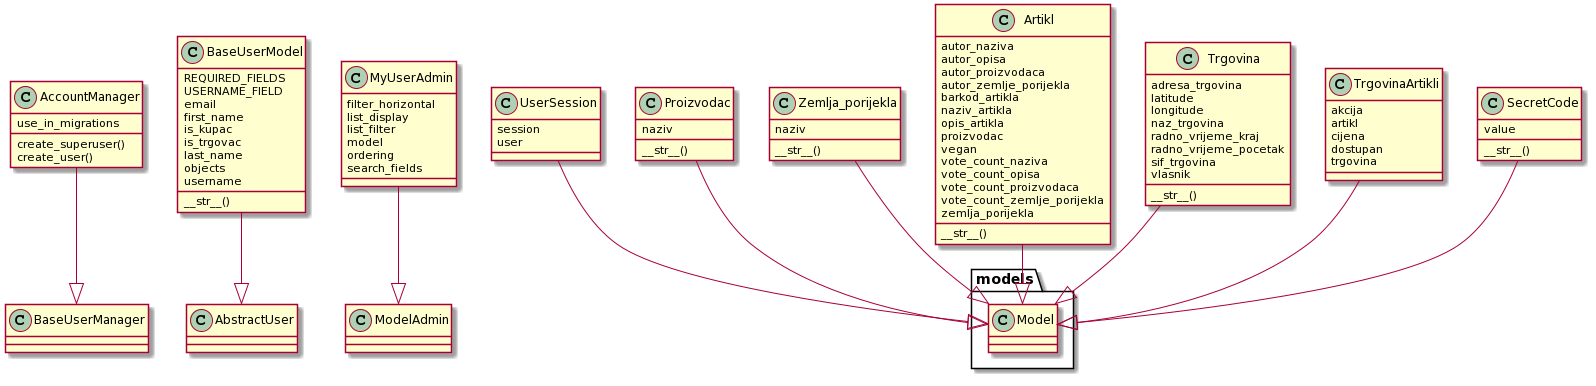
\includegraphics[width=1.0\linewidth]{dijagrami/class_posluzitelj.png}
			\caption{Dijagram razreda na poslužitelju}
			\label{fig:class_posluzitelj}
		\end{figure}
			
			
			
			\eject

